\section{\textbf{Grafici}}
\begin{figure}[h]
\label{fes14}
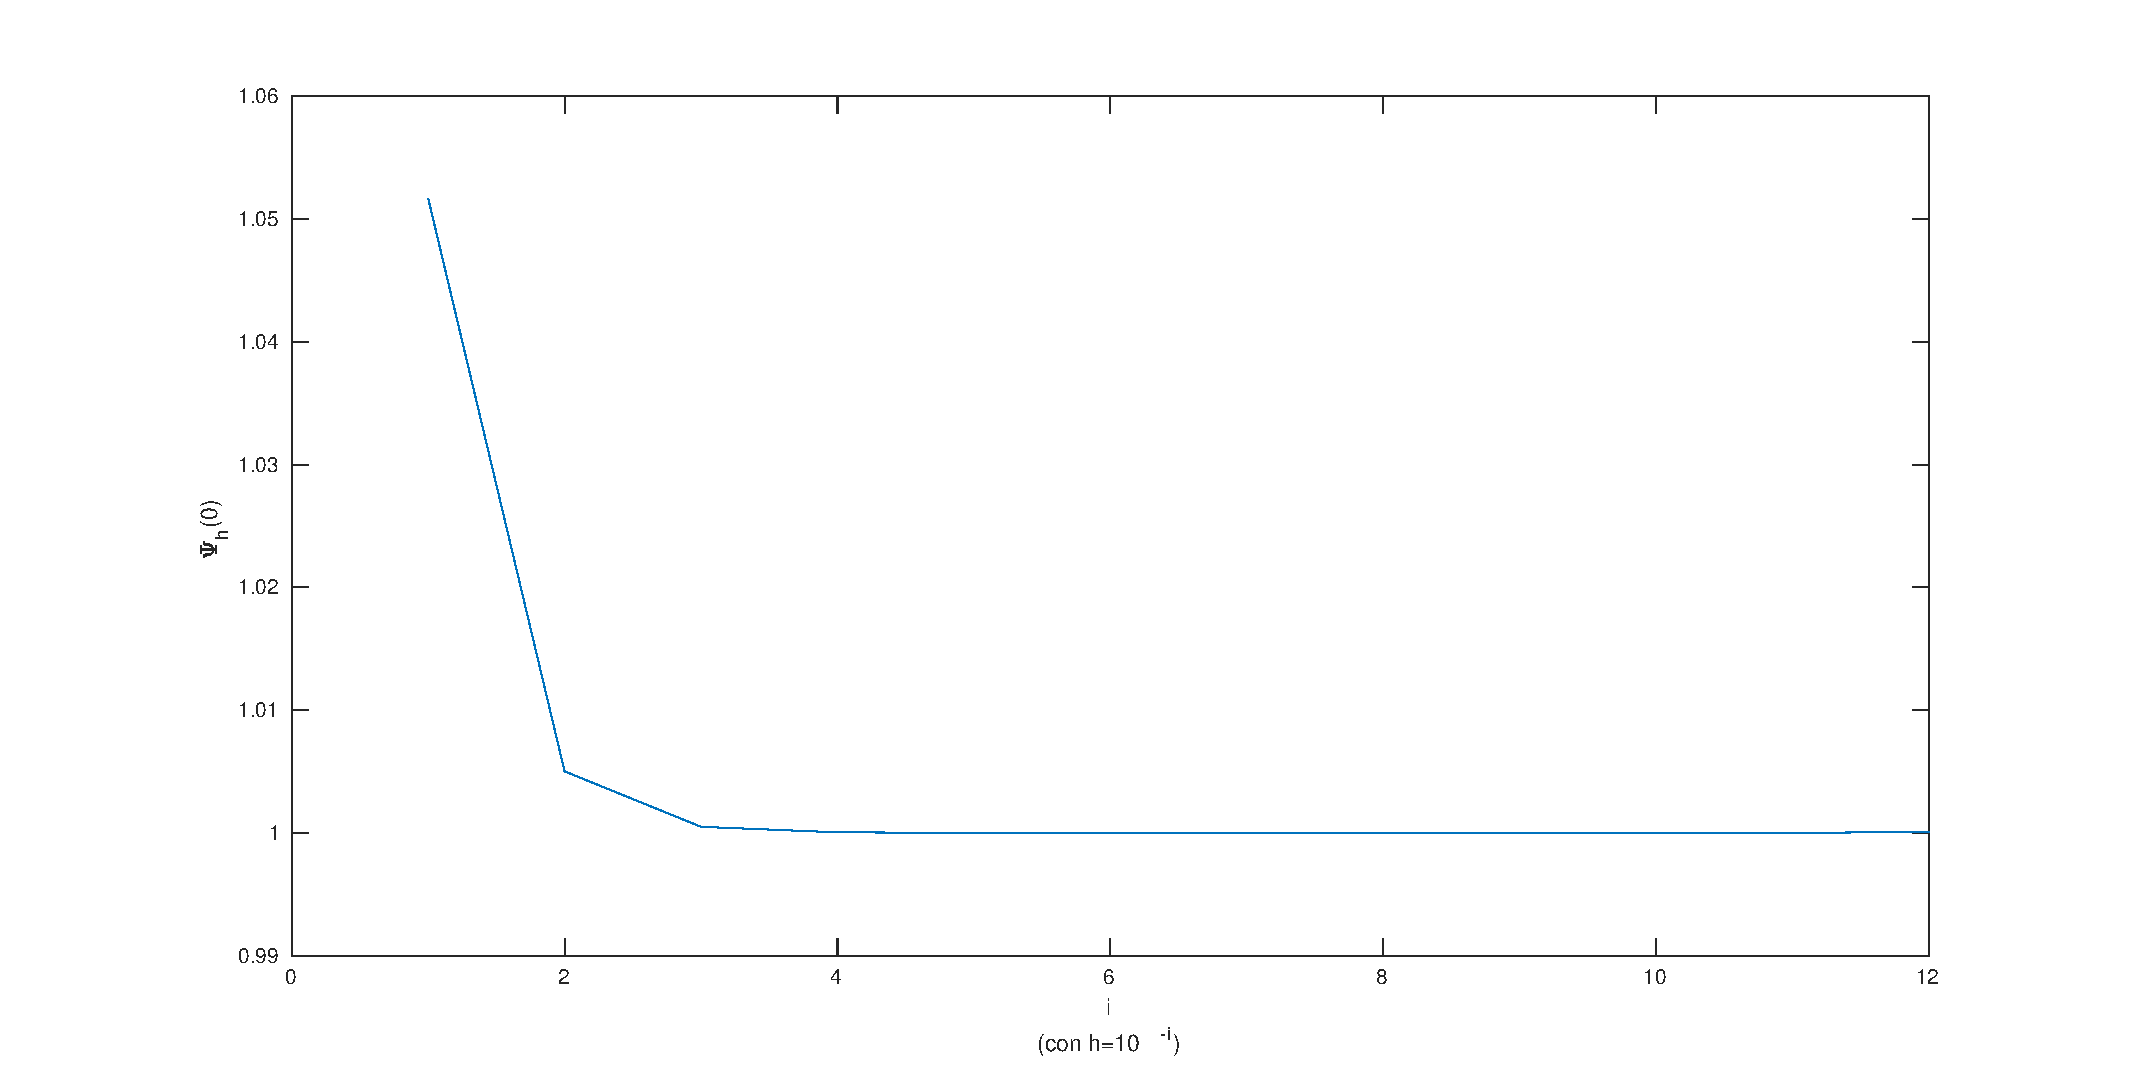
\includegraphics[width=\textwidth]{plot/fes14}
\caption{Andamento della funzione $\Psi_{h}(0)$}
\end{figure}
\begin{figure}[h]
\label{fes113}
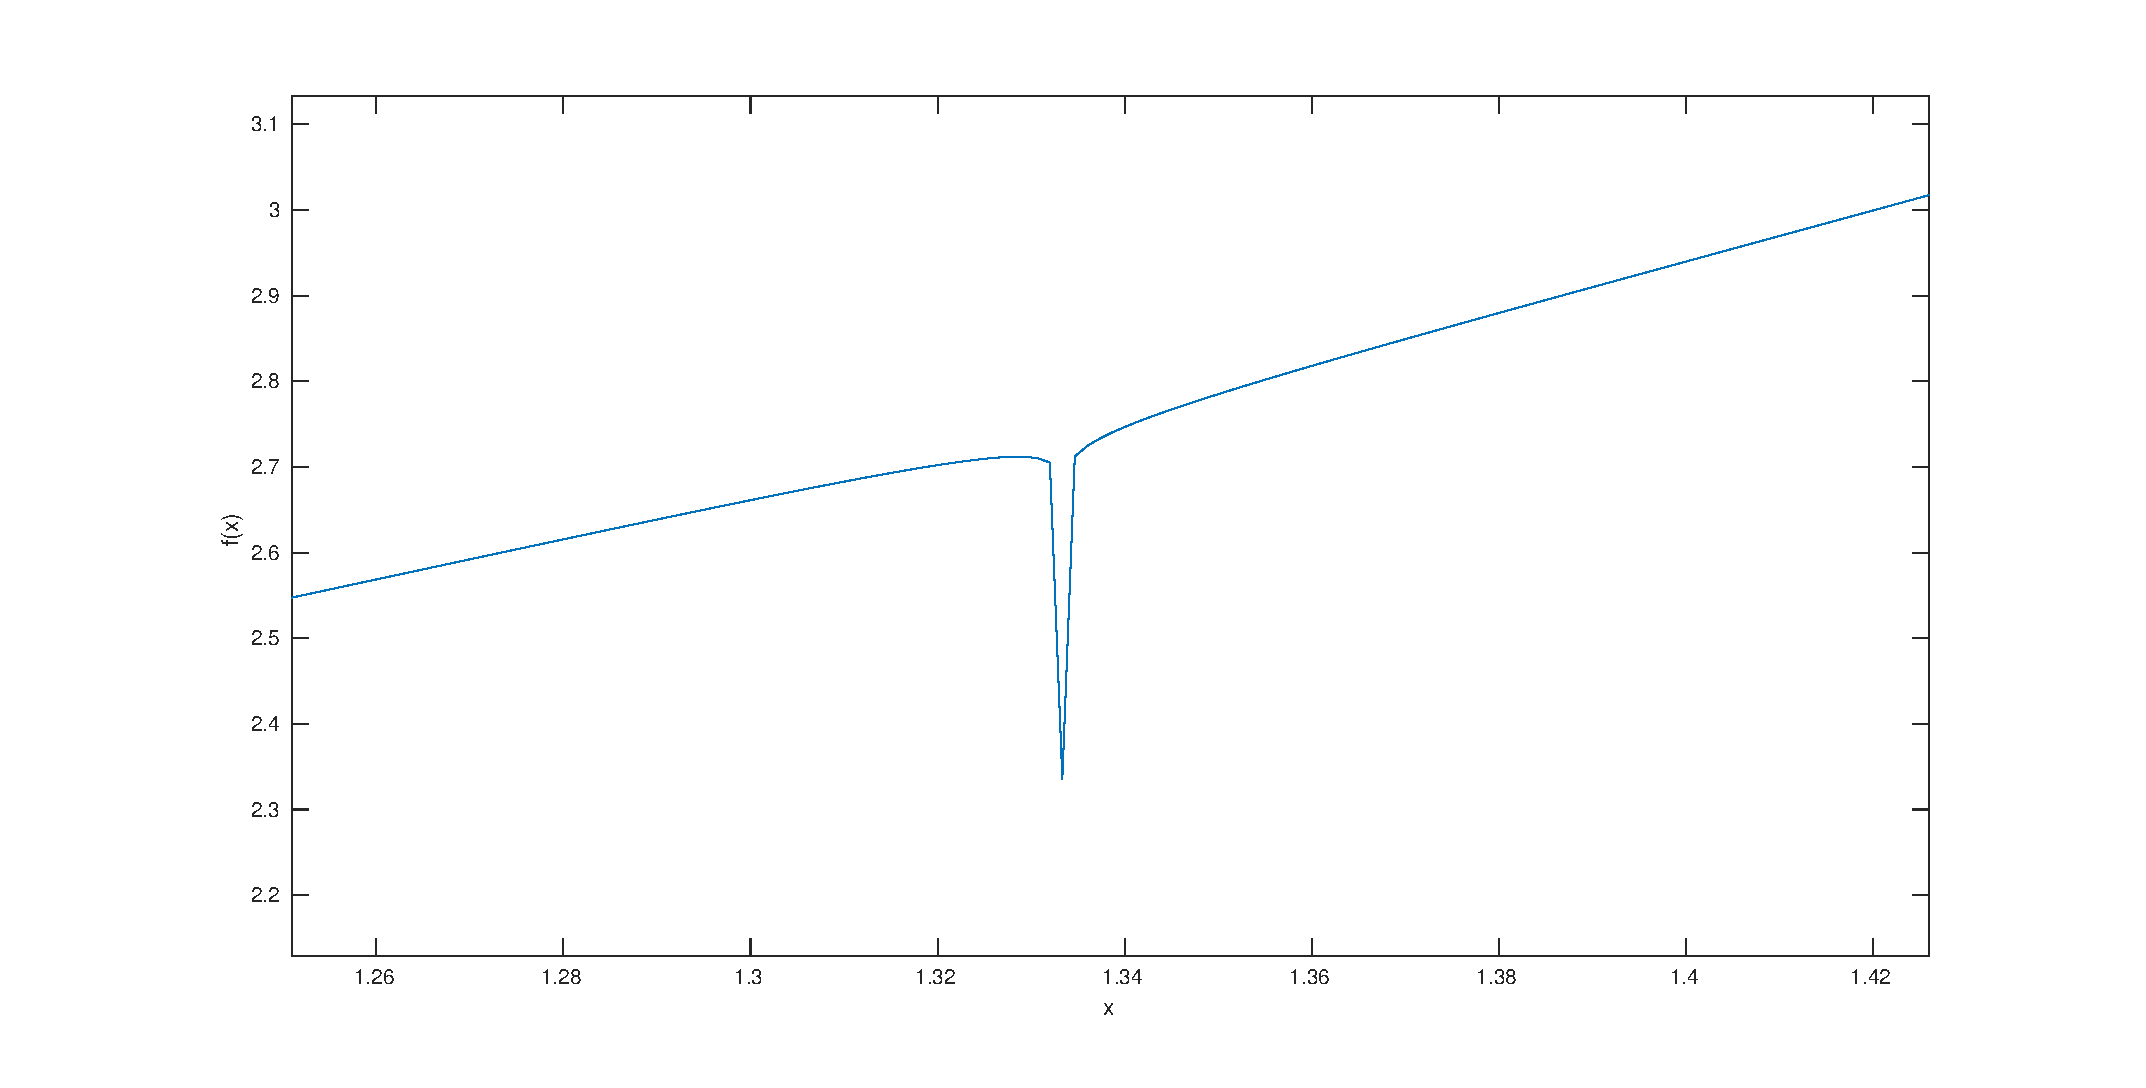
\includegraphics[width=\textwidth]{plot/fes113}
\caption{Plot MatLab della funzione $f(x)=\frac{ln(|3(1-x)+1|)}{80}+x^2+1$}
\end{figure}
\begin{figure}[h]
\label{fes26}
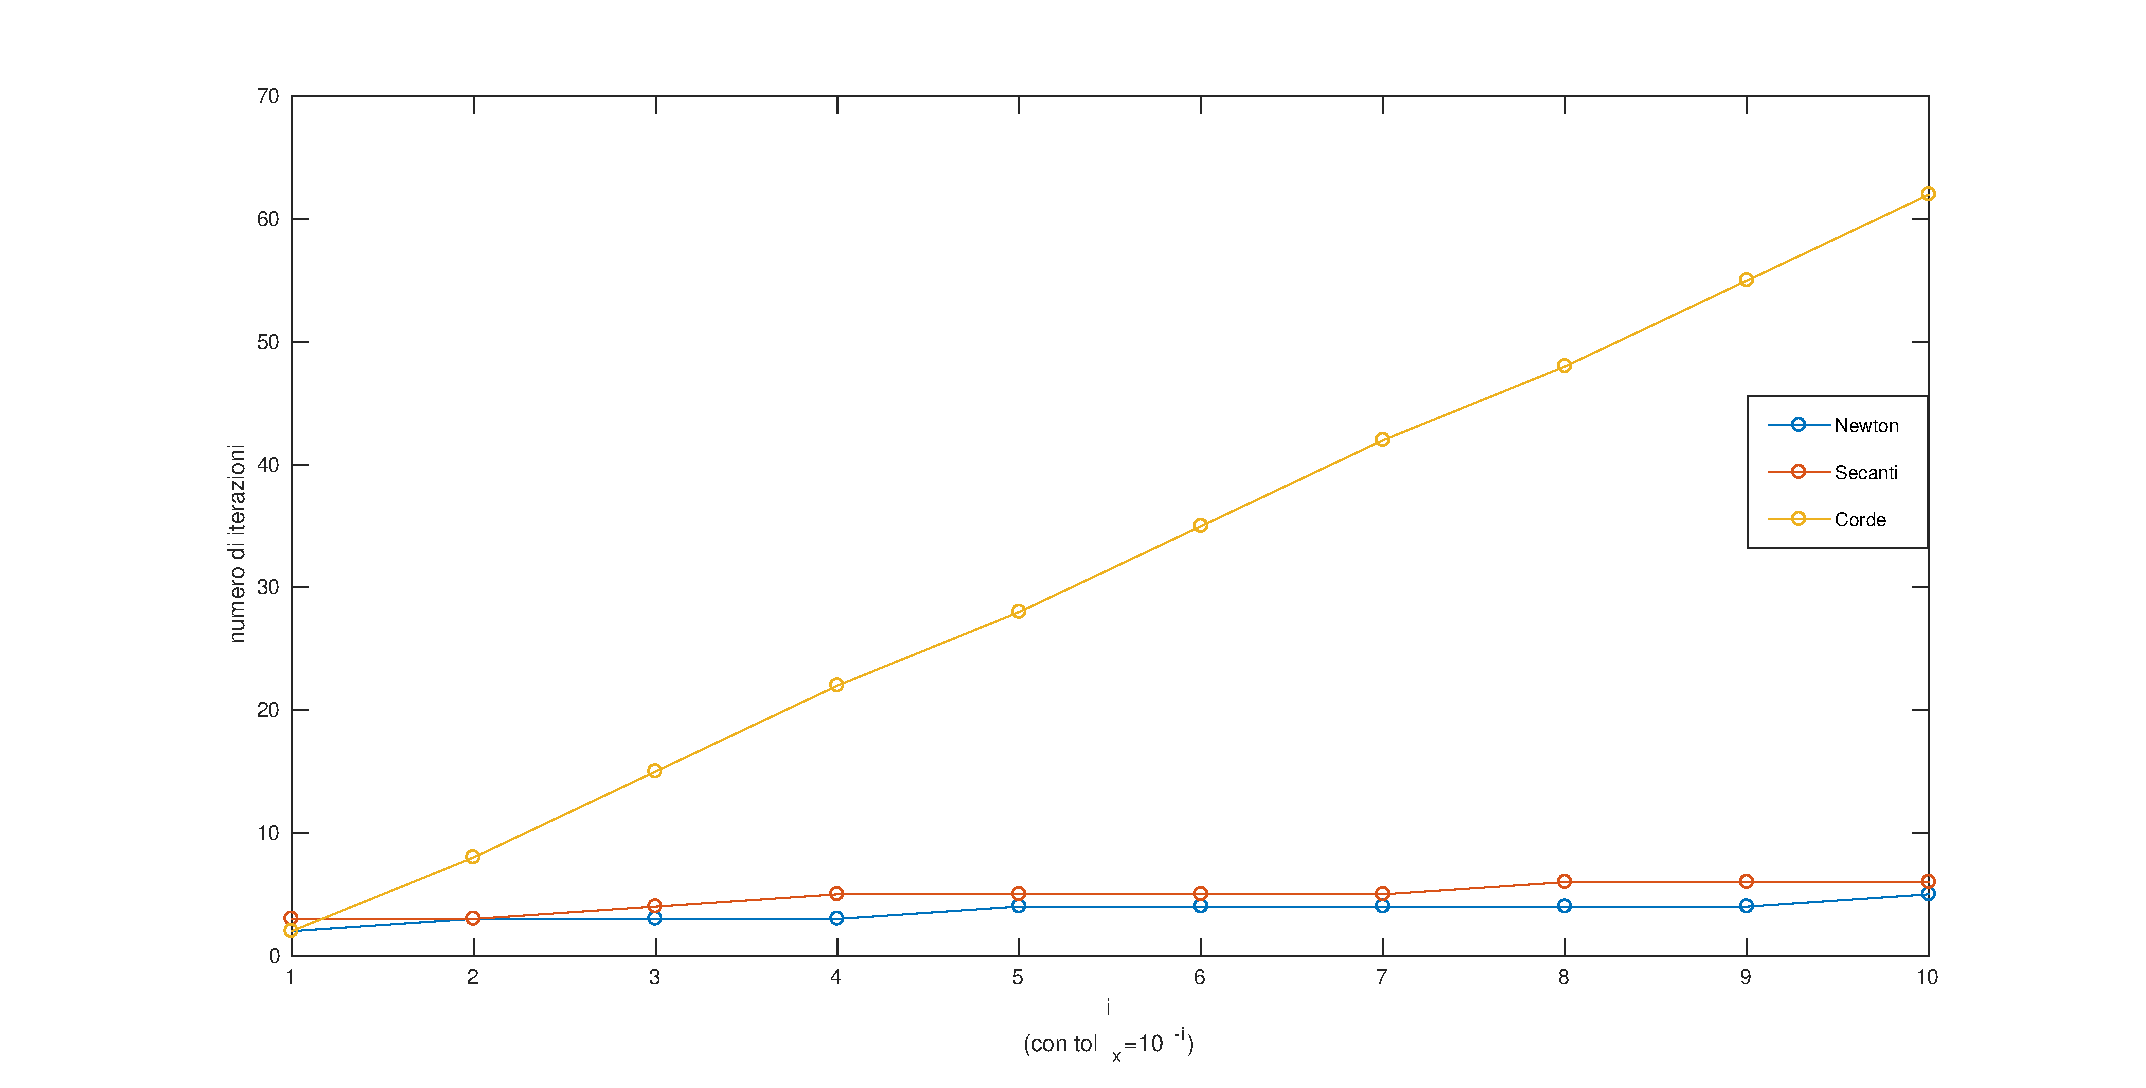
\includegraphics[left, scale=1]{plot/fes26}
\caption{Andamento del numero delle iterazioni al decrescere della tolleranza per i metodi Newton, Secanti, Corde}
\end{figure}
\begin{figure}[h]
\label{fes27}
\includegraphics[left, scale=0.6]{plot/fes27}
\caption{Aggiunta dell'andamento del metodo di Bisezione rispetto ai precedenti metodi}
\end{figure}

%%% 

\begin{figure}[h]
\caption{Runge Chebyshev}
\label{RungeChe}
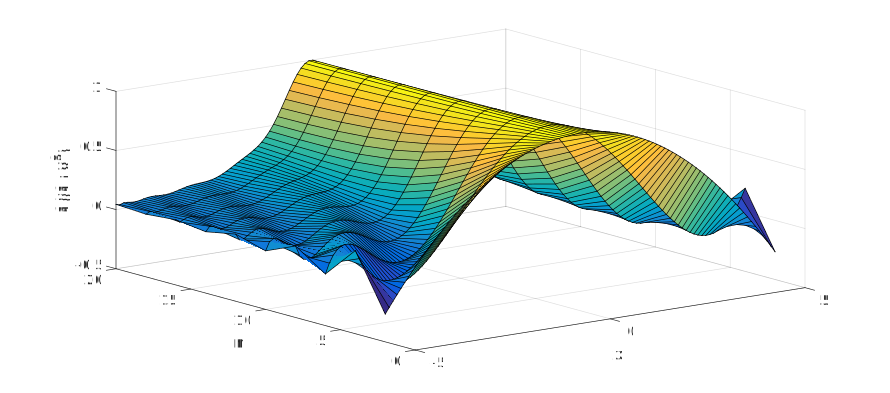
\includegraphics[width=\textwidth]{plot/Runge_cheb}
\end{figure}
\begin{figure}[h]
\caption{Runge Chebyshev Errori}
\label{RungeCheErr}
\includegraphics[width=\textwidth]{plot/Runge_cheb_err}
\end{figure}
\begin{figure}[h]
\caption{Runge con ascisse equidistanti}
\label{RungeEq}
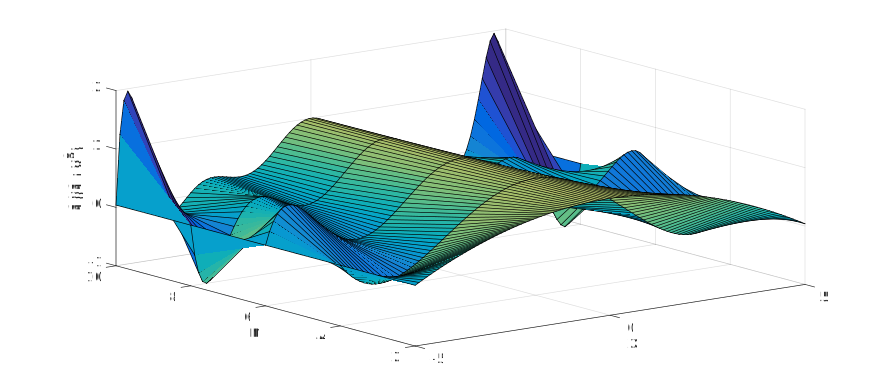
\includegraphics[width=\textwidth]{plot/Runge_equi}
\end{figure}
\begin{figure}[h]
\caption{Runge con ascisse equidistanti errori}
\label{RungeEqErr}
\includegraphics[width=\textwidth]{plot/Runge_equi_err}
\end{figure}
\begin{figure}[h]
\caption{Funzione xsinx Chebyshev}
\label{SinChe}
\includegraphics[width=\textwidth]{plot/Sin_cheb}
\end{figure}
\begin{figure}[h]
\caption{Funzione xsinx Chebyshev errori}
\label{SinCheErr}
\includegraphics[width=\textwidth]{plot/Sin_cheb_Err}
\end{figure}
\begin{figure}[h]
\caption{Funzione xsinx ascisse equidistanti}
\label{SinEq}
\includegraphics[width=\textwidth]{plot/Sin_equi}
\end{figure}
\begin{figure}[h]
\caption{Funzione xsinx ascisse equidistanti errori}
\label{SinEqErr}
\includegraphics[width=\textwidth]{plot/Sin_equi_err}
\end{figure}
\begin{figure}[h]
\caption{Runge not-a-knot}
\label{runge_nak}
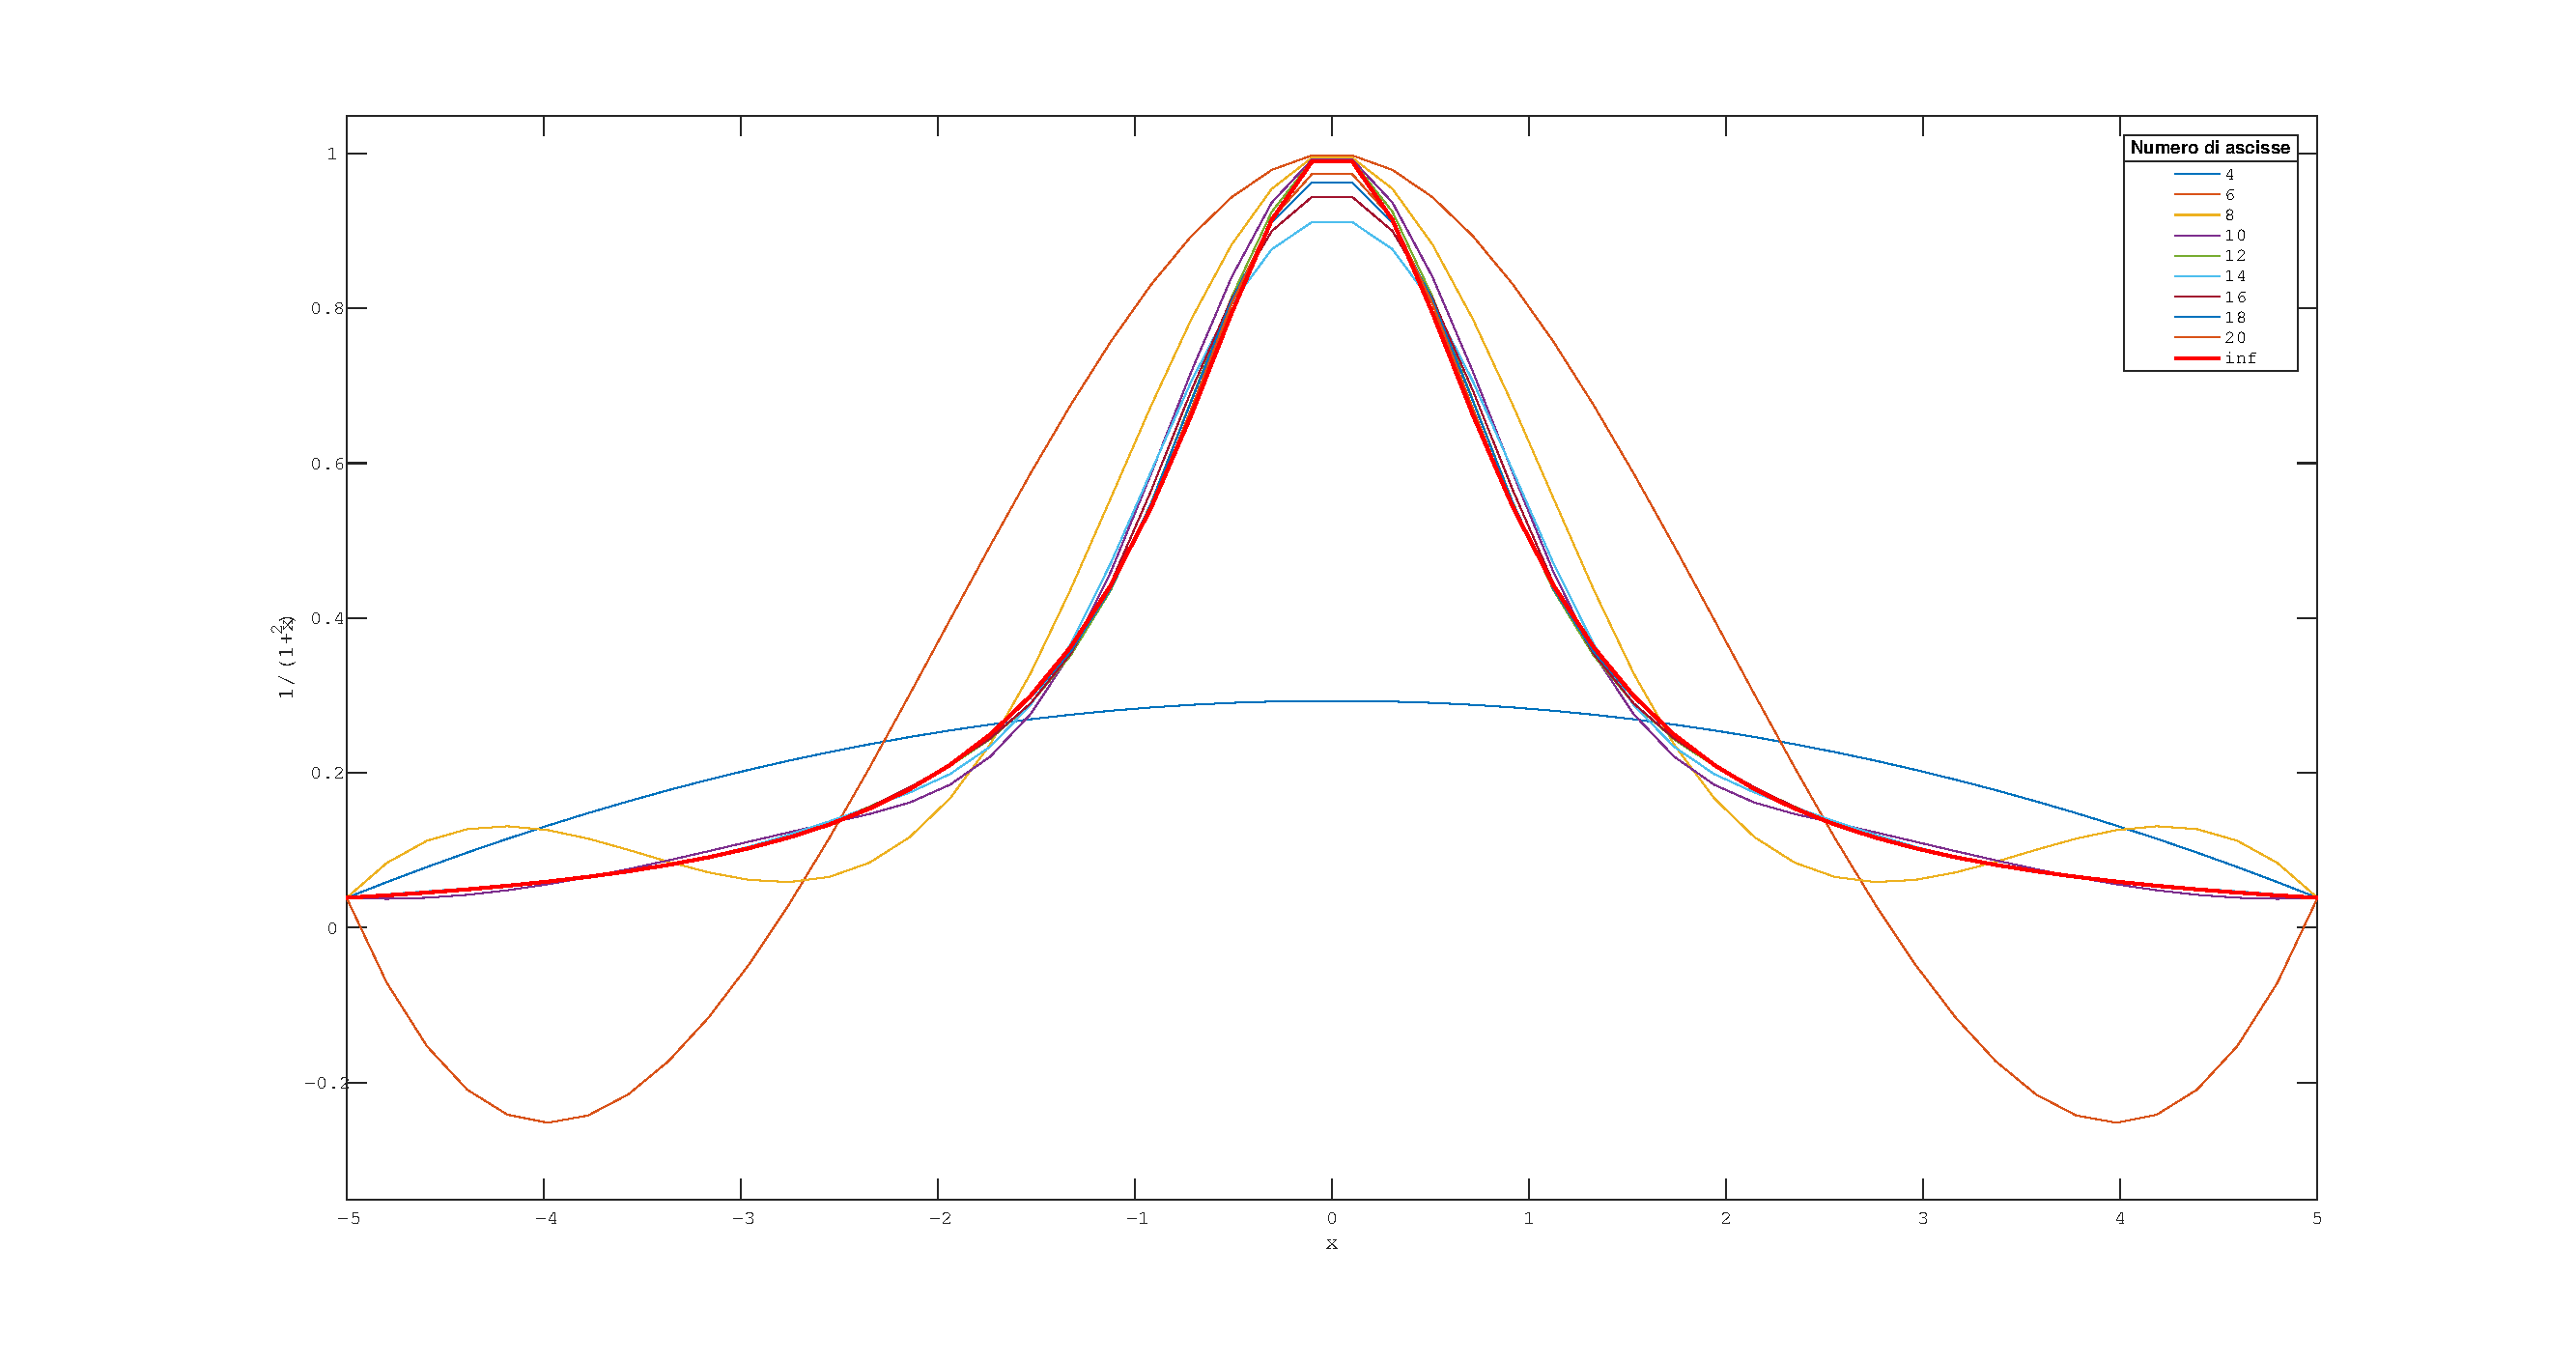
\includegraphics[width=\textwidth]{plot/runge_nak}
\end{figure}
\begin{figure}[h]
\caption{Funzione xsinx not-a-knot}
\label{sin_nak}
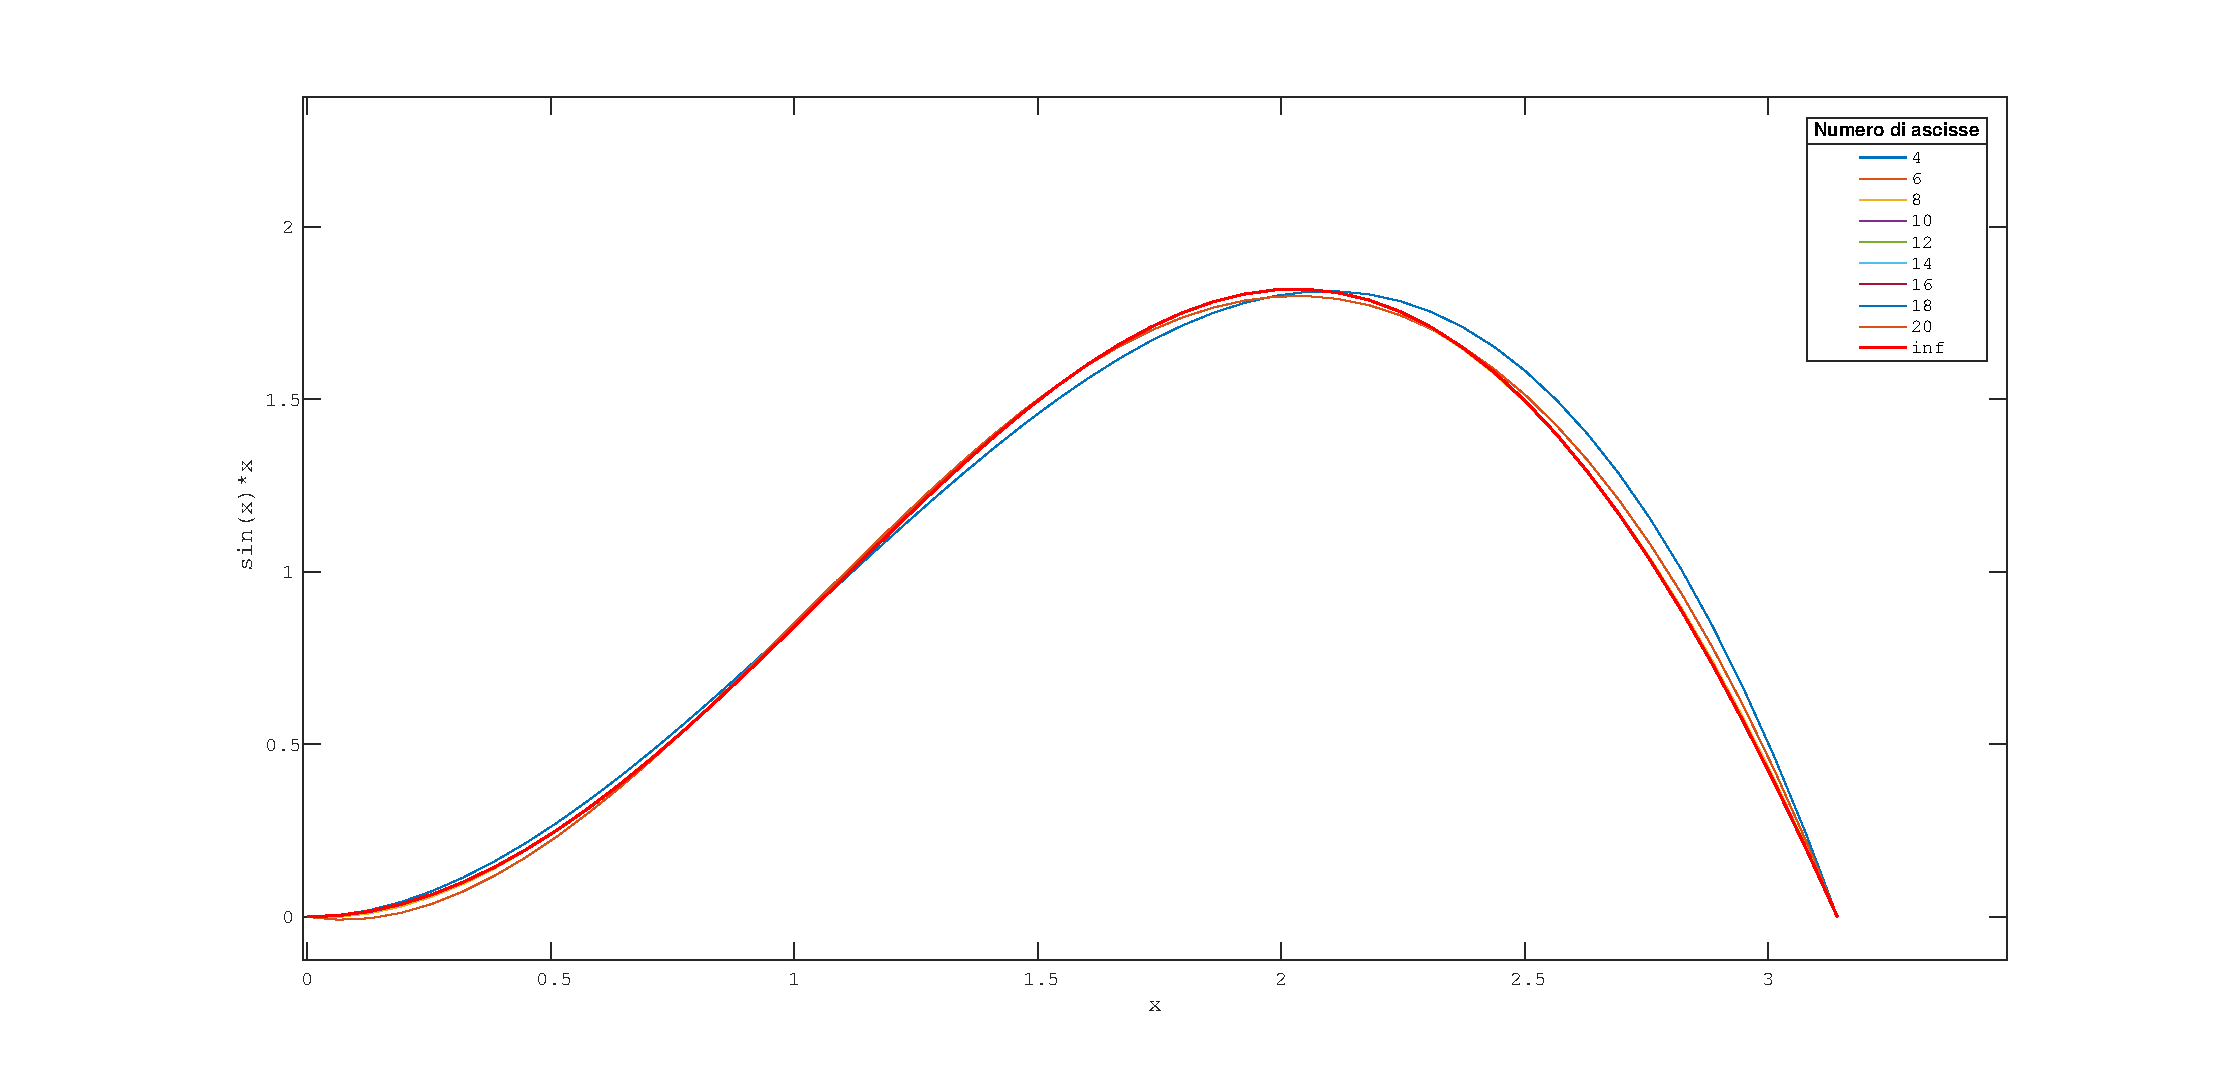
\includegraphics[width=\textwidth]{plot/sin_nak}
\end{figure}
\begin{figure}[h]
\caption{Errori Runge}
\label{erunge_nak}
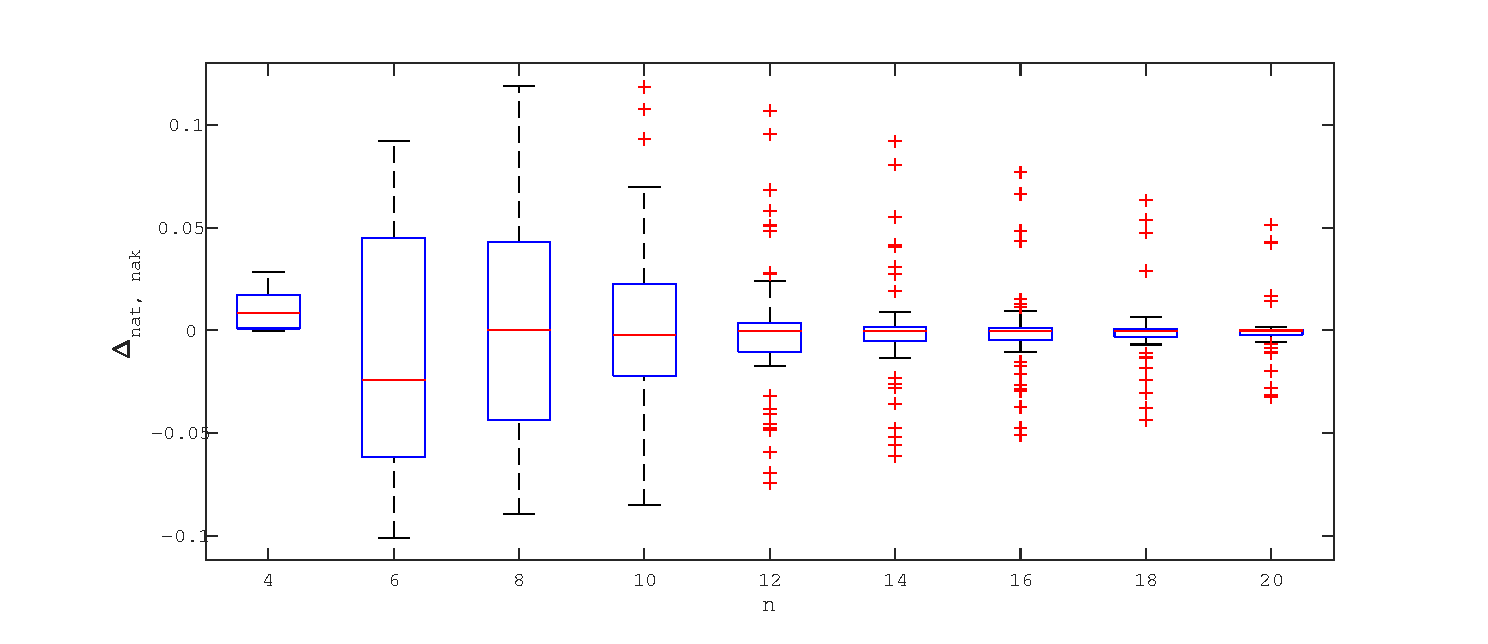
\includegraphics[width=\textwidth]{plot/errors}
\end{figure}
\begin{figure}[h]
\caption{Errori funzione xsinx}
\label{esin_nak}
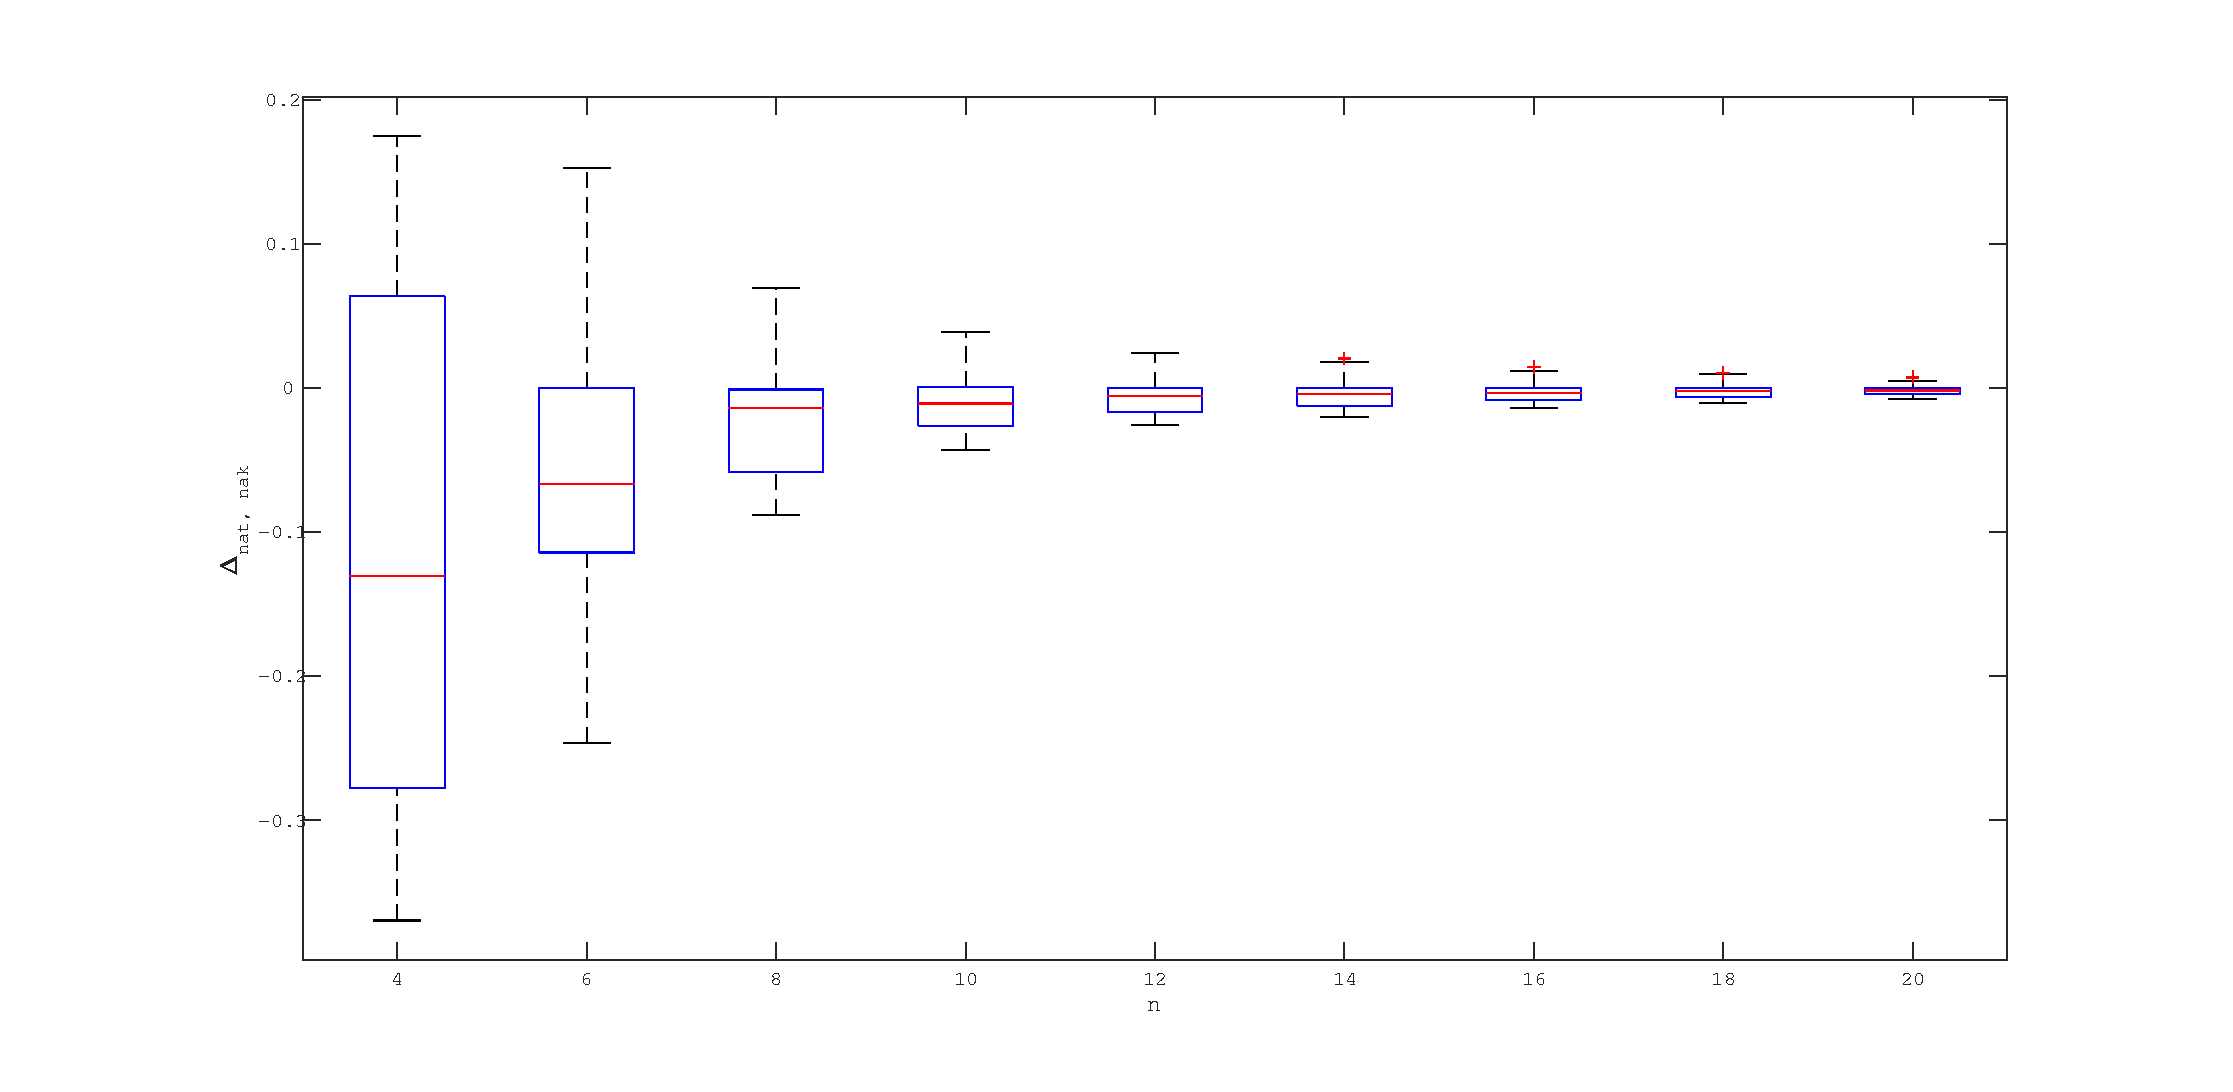
\includegraphics[width=\textwidth]{plot/errors_sin}
\end{figure}
\begin{figure}[h]
\caption{Esercizio 4.10}
\label{fitting}
\includegraphics[width=\textwidth]{plot/fittinginv}
\end{figure}
\begin{figure}[h]
\caption{Esercizio 5.2}
\label{PR_comparison}
\includegraphics[width=\textwidth]{plot/comparison}
\end{figure}
\begin{figure}[h]
\caption{Esercizio 5.2}
\label{QuadrErr}
\includegraphics[width=\textwidth]{plot/error}
\end{figure}
\begin{figure}[h]
\caption{Esercizio 5.6}
\label{QuadrRapp}
\includegraphics[width=\textwidth]{plot/rapp_err}
\end{figure}